%\documentclass[fleqn, letterpaper]{amsart}
\documentclass[fleqn, letterpaper]{tufte-handout}
\usepackage{times}
\usepackage{amsmath}
\usepackage{graphicx}
\usepackage{booktabs}
\usepackage{multirow}
\usepackage{listings}
\usepackage{epstopdf}
\usepackage{bm}
%\usepackage[left=1in]{geometry}

\newcommand{\R}{\mathcal{R}}
\newcommand{\E}{\text{E}}
\newcommand{\p}{p_{XY}}
\renewcommand{\arraystretch}{1.5}

\title{Problem Set 4 --- ENCE689E Spring 2014}
\author{David Prentiss}

\begin{document}
\maketitle

\section{1. Linear Measurement Model}
\subsection{(a)}
For the linear model $z = \alpha_1x_1^2+\alpha_2x_2^2$ we have $\bm{z} = \bm{A}\bm{\alpha}$ where 
\[
        \bm{A} =
        \begin{bmatrix}
                x^2_1 & x^2_2 \\
                \vdots & \vdots \\
                x^2_{N_m} & x^2_{N_m} \\
        \end{bmatrix}
        \quad \text{and} \quad
        \bm{\alpha} =
        \begin{bmatrix}
                \alpha_1 \\ \alpha_2
        \end{bmatrix}
\]
\subsection{(c)}
See Listing \ref{lst1}.
\[
        \hat{\bm{\alpha}} =
        \left[
                \begin{array}{r@{.}l}
                        1&5411 \\ -0&7605
                \end{array}
        \right]
\]
{\small
\begin{minipage}{\linewidth}
        \lstinputlisting[language=Matlab, caption={Monte Carlo estimation of $e^{-x}$ in MATLAB},
        basicstyle=\ttfamily, label=lst1]{problem1.m}
\end{minipage}
}

\subsection{(d)} See Figure \ref{exprnd}
\begin{figure}
        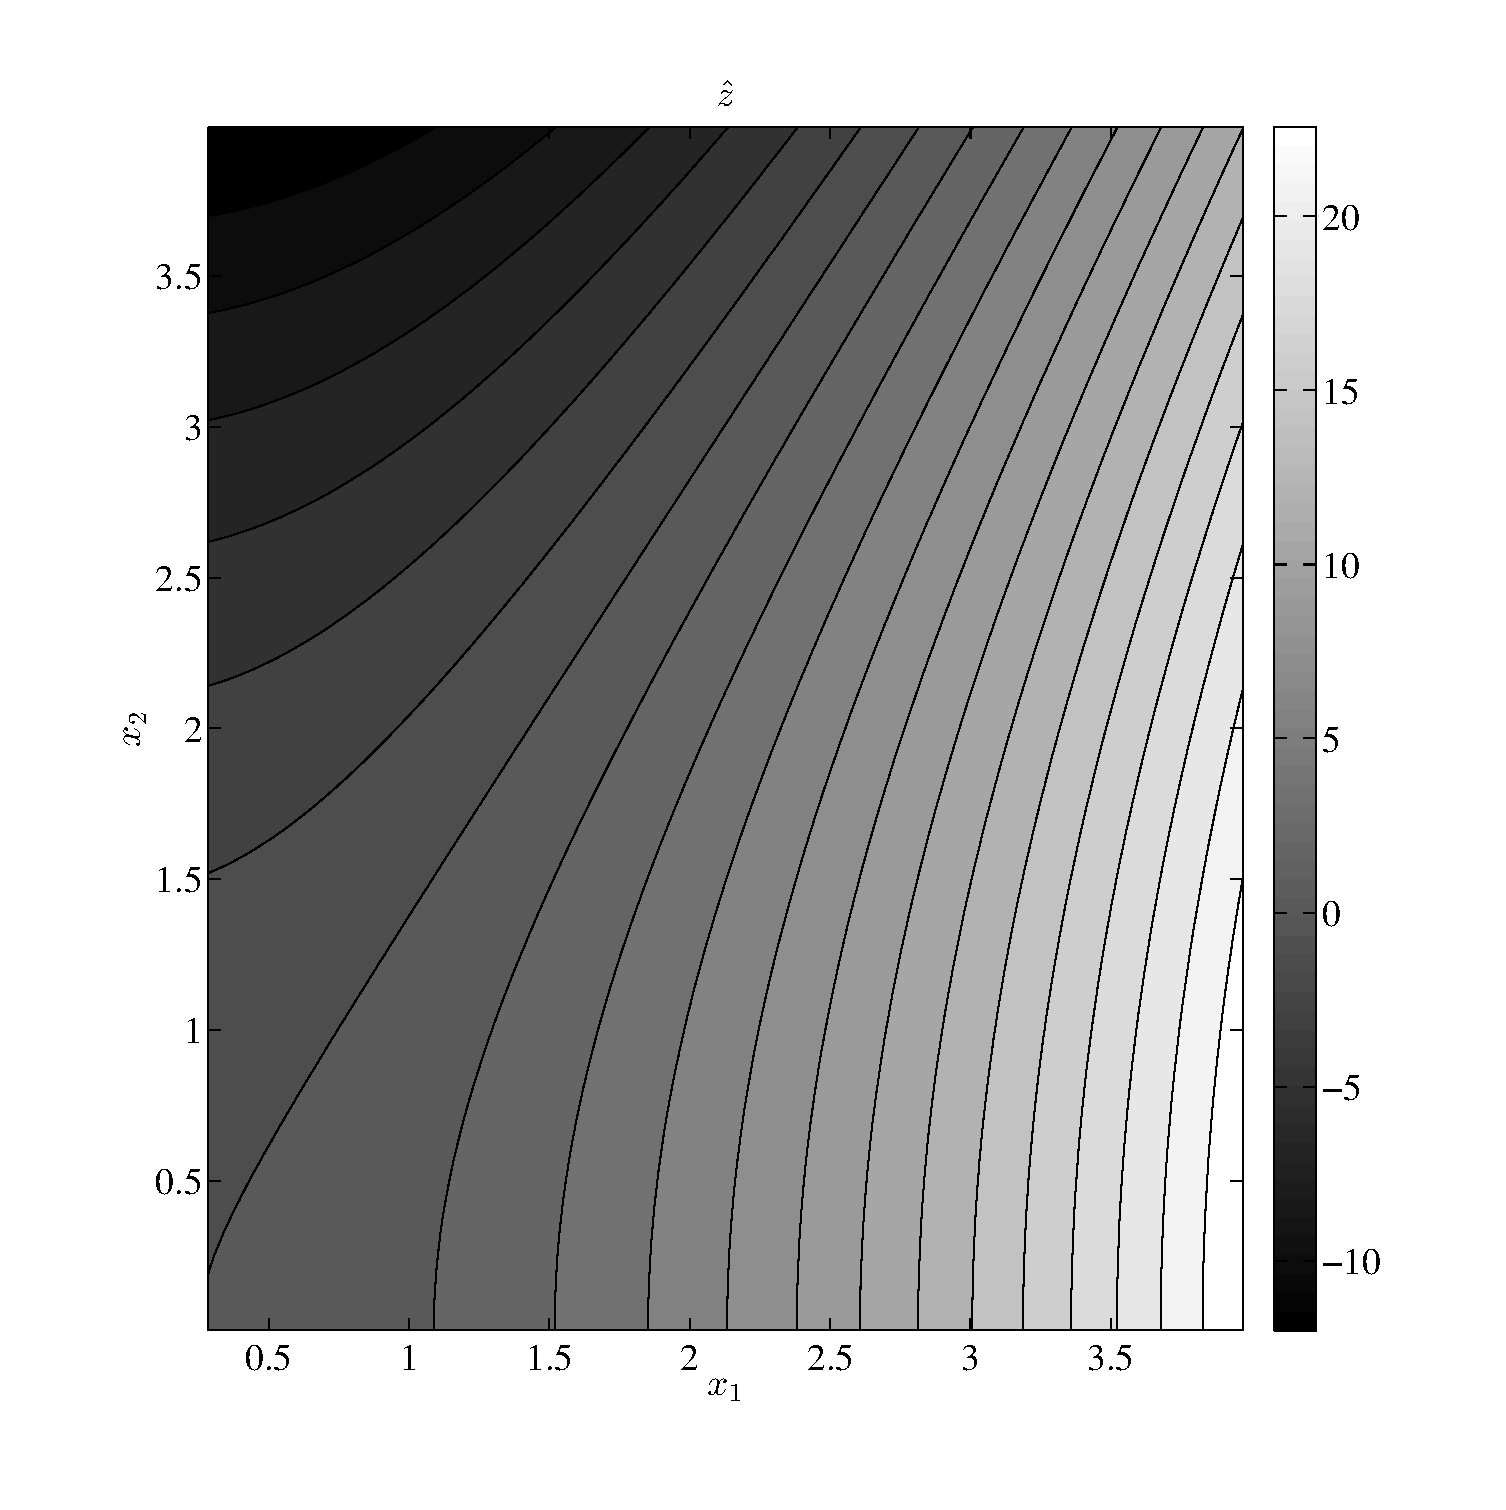
\includegraphics[width=\textwidth]{problem1d}
        \caption{Plot of the predicted field $\hat{z}(x_1,\ x_2)$}
        \label{exprnd}
\end{figure}
\section{Nonlinear Model}
\subsection{(a)}
For the nonlinear model
\[z=\frac{\alpha_1}{\alpha_2 + x}
\]
let the sum of residuals $S$ be
\[S=\sum_1^3\left(z_i-\frac{\alpha_1}{\alpha_2 + x_i}\right)^2
\]
The sum $S$ is minimized for
\[
        \frac{\partial S}{\partial \alpha_1} = 2\sum_1^3\left(z_i-\frac{\alpha_1}{\alpha_2 + x_i}\right)
        \left(\frac{-1}{\alpha_2 + x_i}\right) = 0
\]
\[
        \frac{\partial S}{\partial \alpha_2} = 2\sum_1^3\left(z_i-\frac{\alpha_1}{\alpha_2 + x_i}\right)
        \left(\frac{\alpha_1}{(\alpha_2 + x_i)^{-2}}\right) = 0
\]
\subsection{(b)}
The Gauss-Newton algorithm may be employed to compute $\bm{\alpha}$ iteratively with
\[\bm{\alpha}^{(i+1)} = \bm{\alpha}^{(i)} - (\bm{J}_z^T\bm{J}_z)^{-1}\bm{J}_z^T\bm r \bm{\alpha}^{(i)} 
\]
where $\bm{r}$ is the vector of residuals and the Jacobian $\bm{J}_z$ is
\[
        \bm{J}_z =
        \begin{bmatrix}
                \frac{1}{\alpha_2+x_1} & \frac{-\alpha_1}{(\alpha_2 + x_1)^{-2}} \\
                \frac{1}{\alpha_2+x_2} & \frac{-\alpha_1}{(\alpha_2 + x_2)^{-2}} \\
                \frac{1}{\alpha_2+x_3} & \frac{-\alpha_1}{(\alpha_2 + x_3)^{-2}}
        \end{bmatrix}
\]
\section{Linear Model}
\subsection{(a)}
The mean and variance of the prior as well as the variance of the measurement error are needed to characterize the two random variables.
\subsection{(b)}
\[
        p(\alpha|z) = \frac{p(z|\alpha)p(\alpha)}{p(z)}
        \quad \text{and} \quad
        p(z) = \int p(z|\alpha)p(\alpha)\ d\alpha
\]
\end{document}
